\documentclass[a4paper,12pt,twoside]{article}
%----------------------------------------------------------------------------------------
%	 REQUICouleur8 PACKAGES AND CONFIGURATIONS
%----------------------------------------------------------------------------------------

% Packages nécessaires
\usepackage[french]{babel}
\usepackage[utf8]{inputenc}
\usepackage[T1]{fontenc}
\usepackage{lmodern}
\usepackage{amsmath,amssymb,amsthm}
\usepackage{enumitem}
\setlist[itemize]{label=\raisebox{0.15em}{\scalebox{1}{\textcolor{Couleur8}{$\bullet$}}}, left=1em}
%\setlist[itemize]{label=\textcolor{Couleur6}{\textbullet}, left=1em}
\usepackage{graphicx}
\usepackage{tikz}
\usepackage{tkz-euclide}
\usetikzlibrary{shapes.misc}
\usetikzlibrary{shapes.geometric}
\usetikzlibrary{arrows.meta,shapes.arrows}
\usetikzlibrary{positioning}
\usetikzlibrary{decorations.markings}
\usetikzlibrary{decorations.pathreplacing}
\usepackage{OutilsGeomTikz}
\usetikzlibrary{calc}
\usepackage{pgfplots}
\pgfplotsset{compat=1.18}
\usepackage{multirow}
\usepackage{array}
\usepackage{colortbl}
\usepackage{changepage}
\usepackage{geometry}
\usepackage{fancyhdr}
\usepackage{titlesec}
\usepackage{ProfCollege}
\usepackage{xcolor}
%\usepackage[most]{tcolorbox}
\usepackage{multicol}
\usepackage{amsmath,amsfonts,amssymb,amsthm} 
\usepackage{ifthen} 
\usepackage{titletoc}
% Dans le préambule :
\usepackage{array}
\newcolumntype{C}[1]{>{\centering\arraybackslash}p{#1}}



%----------------------------------------------------------------------------------------
%	 POLICE
%----------------------------------------------------------------------------------------


\renewcommand{\familydefault}{\sfdefault} %Police sans serif
%----------------------------------------------------------------------------------------
%	 COULEURS
%----------------------------------------------------------------------------------------

\definecolor{Couleur1}{HTML}{8b1f30}
\definecolor{Couleur2}{HTML}{725E74}
\definecolor{Couleur3}{HTML}{78985b}
\definecolor{Couleur4}{HTML}{db3e56}
\definecolor{Couleur5}{HTML}{487C4B}
\definecolor{Couleur6}{HTML}{CF6876}
\definecolor{Couleur7}{HTML}{A5C03F} %Vert
\definecolor{Couleur8}{HTML}{D36740} %Orange
\definecolor{Couleur9}{HTML}{7BB48A} %Bleu-Vert
\definecolor{Couleur10}{HTML}{EA8556} %Orange
\definecolor{Couleur11}{HTML}{E6B459} %Jaune
\definecolor{Couleur12}{HTML}{9AC8EB} %Bleu

\definecolor{Bord1}{HTML}{302635}
\definecolor{Bord2}{HTML}{725E74}
\definecolor{Bord3}{HTML}{938999}
\definecolor{Bord4}{HTML}{817888}
\definecolor{Bord5}{HTML}{487C4B}
\definecolor{Bord6}{HTML}{8C436B}
\definecolor{Bord7}{HTML}{A5C03F} %Vert
\definecolor{Bord8}{HTML}{D36740} %Orange

%----------------------------------------------------------------------------------------
%	MARGINS
%----------------------------------------------------------------------------------------

\usepackage{geometry} % RequiCouleur8 for adjusting page dimensions and margins

\geometry{
	top=2cm, % Top margin
	bottom=2cm, % Bottom margin
	inner=2cm, % Inner margin (left on odd pages, right on even or left in oneside mode)
	outer=1.5cm, % Outer margin (right on odd pages, left on even or right in oneside mode)
}



%----------------------------------------------------------------------------------------
%	THEOREM STYLES
%----------------------------------------------------------------------------------------


\newcommand{\intoo}[2]{\mathopen{]}#1\,;#2\mathclose{[}}
\newcommand{\ud}{\mathop{\mathrm{{}d}}\mathopen{}}
\newcommand{\intff}[2]{\mathopen{[}#1\,;#2\mathclose{]}}
\newtheorem{notation}{Notation} 

\newcounter{NumEx}
\setcounter{NumEx}{1}

% Boxed/framed environments
\newtheoremstyle{ocrenumboxTh}% % Theorem style name
{0pt}% Space above
{0pt}% Space below
{\normalfont}% % Body font
{}% Indent amount
{\small\bf\sffamily\color{Couleur1}}% % Theorem head font
{\;}% Punctuation after theorem head
{0.25em}% Space after theorem head
{\small\sffamily\color{Couleur1}\thmname{#1} : % Theorem text (e.g. Theorem 2.1)
\thmnote{\nobreakspace\the\thm@notefont\sffamily\bfseries\color{black}---\nobreakspace#3.}} % Optional theorem note
\renewcommand{\qedsymbol}{$\blacksquare$}% Optional qed square

\newtheoremstyle{ocrenumboxTh*}% % Theorem style name
{0pt}% Space above
{0pt}% Space below
{\normalfont}% % Body font
{}% Indent amount
{\small\bf\sffamily\color{Couleur1}}% % Theorem head font
{\;}% Punctuation after theorem head
{0.25em}% Space after theorem head
{\small\sffamily\color{Couleur1}\thmname{#1} : \\% Theorem text (e.g. Theorem 2.1)
\thmnote{\nobreakspace\the\thm@notefont\sffamily\bfseries\color{black}---\nobreakspace#3.}} % Optional theorem note
\renewcommand{\qedsymbol}{$\blacksquare$}% Optional qed square

\newtheoremstyle{ocrenumboxCoro}% % Theorem style name
{0pt}% Space above
{0pt}% Space below
{\normalfont}% % Body font
{}% Indent amount
{\small\bf\sffamily\color{Couleur1}}% % Theorem head font
{\;}% Punctuation after theorem head
{0.25em}% Space after theorem head
{\small\sffamily\color{Couleur1}\thmname{#1} : % Theorem text (e.g. Theorem 2.1)
\thmnote{\nobreakspace\the\thm@notefont\sffamily\bfseries\color{black}---\nobreakspace#3.}} % Optional theorem note
\renewcommand{\qedsymbol}{$\blacksquare$}% Optional qed square

\newtheoremstyle{ocrenumboxCoro*}% % Theorem style name
{0pt}% Space above
{0pt}% Space below
{\normalfont}% % Body font
{}% Indent amount
{\small\bf\sffamily\color{Couleur1}}% % Theorem head font
{\;}% Punctuation after theorem head
{0.25em}% Space after theorem head
{\small\sffamily\color{Couleur1}\thmname{#1} : \\% Theorem text (e.g. Theorem 2.1)
\thmnote{\nobreakspace\the\thm@notefont\sffamily\bfseries\color{black}---\nobreakspace#3.}} % Optional theorem note
\renewcommand{\qedsymbol}{$\blacksquare$}% Optional qed square


\newtheoremstyle{ocrenumboxNot}% % Theorem style name
{0pt}% Space above
{0pt}% Space below
{\normalfont}% % Body font
{}% Indent amount
{\small\bf\sffamily\color{Couleur8}}% % Theorem head font
{\;}% Punctuation after theorem head
{0.25em}% Space after theorem head
{\small\sffamily\color{Couleur8}\thmname{#1} : % Theorem text (e.g. Theorem 2.1)
\thmnote{\nobreakspace\the\thm@notefont\sffamily\bfseries\color{black}---\nobreakspace#3.}} % Optional theorem note
\renewcommand{\qedsymbol}{$\blacksquare$}% Optional qed square



\newtheoremstyle{ocrenumboxNot*}% % Theorem style name
{0pt}% Space above
{0pt}% Space below
{\normalfont}% % Body font
{}% Indent amount
{\small\bf\sffamily\color{Couleur8}}% % Theorem head font
{\;}% Punctuation after theorem head
{0.25em}% Space after theorem head
{\small\sffamily\color{Couleur8}\thmname{#1} : \\% Theorem text (e.g. Theorem 2.1)
\thmnote{\nobreakspace\the\thm@notefont\sffamily\bfseries\color{black}---\nobreakspace#3.}} % Optional theorem note
\renewcommand{\qedsymbol}{$\blacksquare$}% Optional qed square



\newtheoremstyle{ocrenumboxProp}% % Theorem style name
{0pt}% Space above
{0pt}% Space below
{\normalfont}% % Body font
{}% Indent amount
{\small\bf\sffamily\color{Couleur1}}% % Theorem head font
{\;}% Punctuation after theorem head
{0.25em}% Space after theorem head
{\small\sffamily\color{Couleur1}\thmname{#1} : % Theorem text (e.g. Theorem 2.1)
\thmnote{\nobreakspace\the\thm@notefont\sffamily\bfseries\color{black}---\nobreakspace#3.}} % Optional theorem note
\renewcommand{\qedsymbol}{$\blacksquare$}% Optional qed square



\newtheoremstyle{ocrenumboxProp*}% % Theorem style name
{0pt}% Space above
{0pt}% Space below
{\normalfont}% % Body font
{}% Indent amount
{\small\bf\sffamily\color{Couleur1}}% % Theorem head font
{\;}% Punctuation after theorem head
{0.25em}% Space after theorem head
{\small\sffamily\color{Couleur1}\thmname{#1} : \\% Theorem text (e.g. Theorem 2.1)
\thmnote{\nobreakspace\the\thm@notefont\sffamily\bfseries\color{black}---\nobreakspace#3.}} % Optional theorem note
\renewcommand{\qedsymbol}{$\blacksquare$}% Optional qed square

\newtheoremstyle{ocrenumboxExercice}% % Theorem style name
{0pt}% Space above
{0pt}% Space below
{\normalfont}% % Body font
{}% Indent amount
{\small\bf\sffamily\color{Couleur8}}% % Theorem head font
{\;}% Punctuation after theorem head
{0.25em}% Space after theorem head
{\small\sffamily\color{Couleur8}\thmname{#1}\nobreakspace\theNumEx\addtocounter{NumEx}{1} \,: \\ % Theorem text (e.g. Theorem 2.1)
\thmnote{\nobreakspace\the\thm@notefont\sffamily\bfseries\color{black}---\nobreakspace#3.}} % Optional theorem note
\renewcommand{\qedsymbol}{$\blacksquare$}% Optional qed square

\newtheoremstyle{ocrenumboxEx}% % Theorem style name
{0pt}% Space above
{0pt}% Space below
{\normalfont}% % Body font
{}% Indent amount
{\small\bf\sffamily\color{Couleur8}}% % Theorem head font
{\;}% Punctuation after theorem head
{0.25em}% Space after theorem head
{\small\sffamily\color{Couleur8}\thmname{#1} : \\ % Theorem text (e.g. Theorem 2.1)
\thmnote{\nobreakspace\the\thm@notefont\sffamily\bfseries\color{black}---\nobreakspace#3.}} % Optional theorem note
\renewcommand{\qedsymbol}{$\blacksquare$}% Optional qed square

\newtheoremstyle{ocrenumboxMéthode}% % Theorem style name
{0pt}% Space above
{0pt}% Space below
{\normalfont}% % Body font
{}% Indent amount
{\small\bf\sffamily\color{Couleur7}}% % Theorem head font
{\;}% Punctuation after theorem head
{0.25em}% Space after theorem head
{\small\sffamily\color{Couleur7}\thmname{#1} : % Theorem text (e.g. Theorem 2.1)
\thmnote{\nobreakspace\the\thm@notefont\sffamily\bfseries\color{black}---\nobreakspace#3.}} % Optional theorem note
\renewcommand{\qedsymbol}{$\blacksquare$}% Optional qed square

\newtheoremstyle{ocrenumboxDef}% % Theorem style name
{0pt}% Space above
{0pt}% Space below
{\normalfont}% % Body font
{}% Indent amount
{\small\bf\sffamily\color{Couleur6}}% % Theorem head font
{\;}% Punctuation after theorem head
{0.25em}% Space after theorem head
{\small\sffamily\color{Couleur6}\thmname{#1} : % Theorem text (e.g. Theorem 2.1)
\thmnote{\nobreakspace\the\thm@notefont\sffamily\bfseries\color{black}---\nobreakspace#3.}} % Optional theorem note
\renewcommand{\qedsymbol}{$\blacksquare$}% Optional qed square

\newtheoremstyle{ocrenumboxDef*}% % Theorem style name
{0pt}% Space above
{0pt}% Space below
{\normalfont}% % Body font
{}% Indent amount
{\small\bf\sffamily\color{Couleur6}}% % Theorem head font
{\;}% Punctuation after theorem head
{0.25em}% Space after theorem head
{\small\sffamily\color{Couleur6}\thmname{#1} : \\% Theorem text (e.g. Theorem 2.1)
\thmnote{\nobreakspace\the\thm@notefont\sffamily\bfseries\color{black}---\nobreakspace#3.}} % Optional theorem note
\renewcommand{\qedsymbol}{$\blacksquare$}% Optional qed square


\newtheoremstyle{ocrenumboxReg}% % Theorem style name
{0pt}% Space above
{0pt}% Space below
{\normalfont}% % Body font
{}% Indent amount
{\small\bf\sffamily\color{Couleur6}}% % Theorem head font
{\;}% Punctuation after theorem head
{0.25em}% Space after theorem head
{\small\sffamily\color{Couleur6}\thmname{#1} : % Theorem text (e.g. Theorem 2.1)
\thmnote{\nobreakspace\the\thm@notefont\sffamily\bfseries\color{black}---\nobreakspace#3.}} % Optional theorem note
\renewcommand{\qedsymbol}{$\blacksquare$}% Optional qed square

\newtheoremstyle{ocrenumboxReg*}% % Theorem style name
{0pt}% Space above
{0pt}% Space below
{\normalfont}% % Body font
{}% Indent amount
{\small\bf\sffamily\color{Couleur6}}% % Theorem head font
{\;}% Punctuation after theorem head
{0.25em}% Space after theorem head
{\small\sffamily\color{Couleur6}\thmname{#1} : \\% Theorem text (e.g. Theorem 2.1)
\thmnote{\nobreakspace\the\thm@notefont\sffamily\bfseries\color{black}---\nobreakspace#3.}} % Optional theorem note
\renewcommand{\qedsymbol}{$\blacksquare$}% Optional qed square

\newtheoremstyle{ocrenumboxVoc}% % Theorem style name
{0pt}% Space above
{0pt}% Space below
{\normalfont}% % Body font
{}% Indent amount
{\small\bf\sffamily\color{Couleur3}}% % Theorem head font
{\;}% Punctuation after theorem head
{0.25em}% Space after theorem head
{\small\sffamily\color{Couleur3}\thmname{#1} : \\% Theorem text (e.g. Theorem 2.1)
\thmnote{\nobreakspace\the\thm@notefont\sffamily\bfseries\color{black}---\nobreakspace#3.}} % Optional theorem note
\renewcommand{\qedsymbol}{$\blacksquare$}% Optional qed square

\newtheoremstyle{blacknumex}% Theorem style name
{5pt}% Space above
{5pt}% Space below
{\normalfont}% Body font
{} % Indent amount
{\small\bf\sffamily}% Theorem head font
{\;}% Punctuation after theorem head
{0.25em}% Space after theorem head
{\small\sffamily{\tiny\ensuremath{\blacksquare}}thmname{#1} : % Theorem text (e.g. Theorem 2.1)
\thmnote{\nobreakspace\the\thm@notefont\sffamily\bfseries---\nobreakspace#3.}}% Optional theorem note

\newtheoremstyle{blacknumbox} % Theorem style name
{0pt}% Space above
{0pt}% Space below
{\normalfont}% Body font
{}% Indent amount
{\small\bf\sffamily}% Theorem head font
{\;}% Punctuation after theorem head
{0.25em}% Space after theorem head
{\small\sffamily\thmname{#1} : \\% Theorem text (e.g. Theorem 2.1)
\thmnote{\nobreakspace\the\thm@notefont\sffamily\bfseries---\nobreakspace#3.}}% Optional theorem note

% Non-boxed/non-framed environments
\newtheoremstyle{ocrenum}% % Theorem style name
{5pt}% Space above
{5pt}% Space below
{\normalfont}% % Body font
{}% Indent amount
{\small\bf\sffamily\color{Orange}}% % Theorem head font
{\;}% Punctuation after theorem head
{0.25em}% Space after theorem head
{\small\sffamily\color{Orange}\thmname{#1} : \\% Theorem text (e.g. Theorem 2.1)
\thmnote{\nobreakspace\the\thm@notefont\sffamily\bfseries\color{black}---\nobreakspace#3.}} % Optional theorem note
\renewcommand{\qedsymbol}{$\blacksquare$}% Optional qed square
\makeatother

% Defines the theorem text style for each type of theorem to one of the three styles above
\newcounter{dummy} 
\numberwithin{dummy}{section}
\theoremstyle{ocrenumboxTh}
\newtheorem{problem}{Problem} 
\theoremstyle{ocrenumboxExercice}
\newtheorem{exerciseT}{Exercice} 
\theoremstyle{ocrenumboxExercice}
\newtheorem{exercisesT}{Exercices} 
\theoremstyle{ocrenumboxEx}
\newtheorem{exampleT}{Exemple} 
\theoremstyle{ocrenumboxEx}
\newtheorem{examplesT}{Exemples} 

\theoremstyle{ocrenumboxTh}
\newtheorem{theoremeT}[dummy]{Théorème}
\theoremstyle{ocrenumboxTh*}
\newtheorem{theoremeT*}[dummy]{Théorème}

\theoremstyle{ocrenumboxTh}
\newtheorem{theoremesT}[dummy]{Théorèmes}
\theoremstyle{ocrenumboxTh*}
\newtheorem{theoremesT*}[dummy]{Théorèmes}


\theoremstyle{ocrenumboxCoro}
\newtheorem{corollaryT}[dummy]{Corollaire}
\theoremstyle{ocrenumboxCoro*}
\newtheorem{corollaryT*}[dummy]{Corollaire}

\theoremstyle{ocrenumboxCoro}
\newtheorem{corollarysT}[dummy]{Corollaires}
\theoremstyle{ocrenumboxCoro*}
\newtheorem{corollarysT*}[dummy]{Corollaires}


\theoremstyle{ocrenumboxProp}
\newtheorem{proposition}[dummy]{Propriété}
\theoremstyle{ocrenumboxProp*}
\newtheorem{proposition*}[dummy]{Propriété}

\theoremstyle{ocrenumboxProp}
\newtheorem{propositions}[dummy]{Propriétés}
\theoremstyle{ocrenumboxProp*}
\newtheorem{propositions*}[dummy]{Propriétés}


\theoremstyle{ocrenumboxMéthode}
\newtheorem{methode}[dummy]{Méthode}

\theoremstyle{ocrenumboxMéthode}
\newtheorem{methodes}[dummy]{Méthodes}


\theoremstyle{ocrenumboxDef}
\newtheorem{definitionT}{Définition}[section]
\theoremstyle{ocrenumboxDef*}
\newtheorem{definitionT*}{Définition}[section]


\theoremstyle{ocrenumboxDef}
\newtheorem{definitionsT}{Définitions}[section]
\theoremstyle{ocrenumboxDef*}
\newtheorem{definitionsT*}{Définitions}[section]


\theoremstyle{ocrenumboxReg}
\newtheorem{regleT}{Règle}[section]
\theoremstyle{ocrenumboxReg*}
\newtheorem{regleT*}{Règle}[section]



\theoremstyle{ocrenumboxReg}
\newtheorem{reglesT}{Règles}[section]
\theoremstyle{ocrenumboxReg*}
\newtheorem{reglesT*}{Règles}[section]


\theoremstyle{ocrenumboxVoc}
\newtheorem{vocabulary}{Vocabulaire} 
\theoremstyle{ocrenumboxVoc}
\newtheorem{vocabularys}{Vocabulaires} 

\theoremstyle{ocrenumboxNot}
\newtheorem{notationM}[dummy]{Notation}
\theoremstyle{ocrenumboxNot}
\newtheorem{notationsM}[dummy]{Notations}

\theoremstyle{ocrenumboxNot*}
\newtheorem{notationM*}[dummy]{Notation}
\theoremstyle{ocrenumboxNot*}
\newtheorem{notationsM*}[dummy]{Notations}

\theoremstyle{ocrenum}


%----------------------------------------------------------------------------------------
%	DEFINITION OF COLOR BOXES
%----------------------------------------------------------------------------------------

\RequirePackage[framemethod=default]{mdframed} % RequiCouleur8 for creating the theorem, definition, exercise and corollary boxes

% Theorem box
\newmdenv[skipabove=7pt,
skipbelow=7pt,
rightline=false,
leftline=true,
topline=false,
bottomline=false,
linecolor=Couleur1,
backgroundcolor=Couleur1!5,
innerleftmargin=5pt,
innerrightmargin=5pt,
innertopmargin=5pt,
leftmargin=0cm,
rightmargin=0cm,
linewidth=4pt,
innerbottommargin=5pt]{tBox}

% Exercise box	  
\newmdenv[skipabove=7pt,
skipbelow=7pt,
rightline=false,
leftline=true,
topline=false,
bottomline=false,
linecolor=Couleur8,
innerleftmargin=5pt,
innerrightmargin=5pt,
innertopmargin=5pt,
innerbottommargin=5pt,
leftmargin=0cm,
rightmargin=0cm,
linewidth=2.5pt]{eBox}	

% Méthode box	  
\newmdenv[skipabove=7pt,
skipbelow=7pt,
rightline=false,
leftline=true,
topline=false,
bottomline=false,
backgroundcolor=Couleur7!10,
linecolor=Couleur7,
innerleftmargin=5pt,
innerrightmargin=5pt,
innertopmargin=5pt,
innerbottommargin=5pt,
leftmargin=0cm,
rightmargin=0cm,
linewidth=4pt]{mBox}	

% Exemple box	  
\newmdenv[skipabove=7pt,
skipbelow=7pt,
rightline=false,
leftline=true,
topline=false,
bottomline=false,
linecolor=Couleur8,
innerleftmargin=5pt,
innerrightmargin=5pt,
innertopmargin=5pt,
innerbottommargin=5pt,
leftmargin=0cm,
rightmargin=0cm,
linewidth=2.5pt]{exBox}	

% Definition box
\newmdenv[skipabove=7pt,
skipbelow=7pt,
rightline=false,
leftline=true,
topline=false,
bottomline=false,
linecolor=Couleur6,
backgroundcolor=Couleur6!10,
innerleftmargin=5pt,
innerrightmargin=5pt,
innertopmargin=5pt,
leftmargin=0cm,
rightmargin=0cm,
linewidth=4pt,
innerbottommargin=5pt]{dBox}	

% Corollary box
\newmdenv[skipabove=7pt,
skipbelow=7pt,
rightline=false,
leftline=true,
topline=false,
bottomline=false,
linecolor=Couleur1,
backgroundcolor=Couleur1!5,
innerleftmargin=5pt,
innerrightmargin=5pt,
innertopmargin=5pt,
leftmargin=0cm,
rightmargin=0cm,
linewidth=4pt,
innerbottommargin=5pt]{cBox}


% Notation box
\newmdenv[skipabove=7pt,
skipbelow=7pt,
rightline=false,
leftline=true,
topline=false,
bottomline=false,
linecolor=Couleur8,
backgroundcolor=Couleur8!10,
innerleftmargin=5pt,
innerrightmargin=5pt,
innertopmargin=5pt,
leftmargin=0cm,
rightmargin=0cm,
linewidth=2pt,
innerbottommargin=5pt]{nBox}

% Vocabulaire box
\newmdenv[skipabove=7pt,
skipbelow=7pt,
rightline=false,
leftline=true,
topline=false,
bottomline=false,
linecolor=Couleur3,
innerleftmargin=5pt,
innerrightmargin=5pt,
innertopmargin=5pt,
leftmargin=0cm,
rightmargin=0cm,
linewidth=2pt,
innerbottommargin=5pt]{vBox}

% Creates an environment for each type of theorem and assigns it a theorem text style from the "Theorem Styles" section above and a coloCouleur8 box from above
\newenvironment{Théorème}{\begin{tBox}\begin{theoremeT}}{\end{theoremeT}\end{tBox}}
\newenvironment{Théorème*}{\begin{tBox}\begin{theoremeT*}}{\end{theoremeT*}\end{tBox}}
\newenvironment{Exercice}{\begin{eBox}\begin{exerciseT}}{\hfill{\color{Couleur8}\tiny\ensuremath{\blacksquare}}\end{exerciseT}\end{eBox}}		
\newenvironment{Théorèmes}{\begin{tBox}\begin{theoremesT}}{\end{theoremesT}\end{tBox}}
\newenvironment{Théorèmes*}{\begin{tBox}\begin{theoremesT*}}{\end{theoremesT*}\end{tBox}}
\newenvironment{Exercices}{\begin{eBox}\begin{exercisesT}}{\hfill{\color{Couleur4}\tiny\ensuremath{\blacksquare}}\end{exercisesT}\end{eBox}}		
\newenvironment{Méthode}{\begin{mBox}\begin{methode}}{\hfill{\color{Couleur7}\tiny\ensuremath{\blacksquare}}\end{methode}\end{mBox}}		
		 
		 \newenvironment{Méthodes}{\begin{mBox}\begin{methodes}}{\hfill{\color{Couleur7}\tiny\ensuremath{\blacksquare}}\end{methodes}\end{mBox}}	
		  
\newenvironment{Définition}{\begin{dBox}\begin{definitionT}}{\end{definitionT}\end{dBox}}	
\newenvironment{Définition*}{\begin{dBox}\begin{definitionT*}}{\end{definitionT*}\end{dBox}}	

\newenvironment{Définitions}{\begin{dBox}\begin{definitionsT}}{\end{definitionsT}\end{dBox}}	
\newenvironment{Définitions*}{\begin{dBox}\begin{definitionsT*}}{\end{definitionsT*}\end{dBox}}	


\newenvironment{Règle}{\begin{dBox}\begin{regleT}}{\end{regleT}\end{dBox}}	
\newenvironment{Règle*}{\begin{dBox}\begin{regleT*}}{\end{regleT*}\end{dBox}}	

\newenvironment{Règles}{\begin{dBox}\begin{reglesT}}{\end{reglesT}\end{dBox}}	
\newenvironment{Règles*}{\begin{dBox}\begin{reglesT*}}{\end{reglesT*}\end{dBox}}	

%\newenvironment{Exemple}{\begin{exBox}\begin{exampleT}}{\hfill{\color{Couleur2}\tiny\ensuremath{\blacksquare}}\end{exampleT}\end{exBox}}
		
		
\newenvironment{Exemple}
  {%
   \par\vspace{2pt}% espace avant le titre
   {\sffamily\bfseries\color{Couleur8} Exemple} % le titre au-dessus
   \par\vspace{0pt}% espace après le titre
   \begin{exBox}%
  }
  {\hfill{\color{Couleur8}\tiny\ensuremath{\blacksquare}}\end{exBox}}
  
  \newenvironment{Exemples}
  {%
   \par\vspace{2pt}% espace avant le titre
   {\sffamily\bfseries\color{Couleur8} Exemples} % le titre au-dessus
   \par\vspace{0pt}% espace après le titre
   \begin{exBox}%
  }
  {\hfill{\color{Couleur8}\tiny\ensuremath{\blacksquare}}\end{exBox}}
  
  
  
  \newenvironment{Notation}{\begin{nBox}\begin{notationM}}{\end{notationM}\end{nBox}}
    \newenvironment{Notations}{\begin{nBox}\begin{notationsM}}{\end{notationsM}\end{nBox}}
    
      \newenvironment{Notation*}{\begin{nBox}\begin{notationM*}}{\end{notationM*}\end{nBox}}
    \newenvironment{Notations*}{\begin{nBox}\begin{notationsM*}}{\end{notationsM*}\end{nBox}}    
    
      \newenvironment{Vocabulaire}{\begin{vBox}\begin{vocabularys}}{\end{vocabularys}\end{vBox}}
    \newenvironment{Vocabulaires}{\begin{vBox}\begin{vocabularys}}{\end{vocabularys}\end{vBox}}
    
  \newenvironment{Vocabulaire*}{\begin{vBox}\begin{notationM*}}{\end{notationM*}\end{vBox}}
    \newenvironment{Vocabulaires*}{\begin{vBox}\begin{notationsM*}}{\end{notationsM*}\end{vBox}}    
    
\newenvironment{Corollaire}{\begin{cBox}\begin{corollaryT}}{\end{corollaryT}\end{cBox}}	
\newenvironment{Corollaire*}{\begin{cBox}\begin{corollaryT*}}{\end{corollaryT*}\end{cBox}}	
\newenvironment{Corollaires}{\begin{cBox}\begin{corollarysT}}{\end{corollarysT}\end{cBox}}	
\newenvironment{Corollaires*}{\begin{cBox}\begin{corollarysT*}}{\end{corollarysT*}\end{cBox}}	
\newenvironment{Propriété}{\begin{cBox}\begin{proposition}}{\end{proposition}\end{cBox}}	
\newenvironment{Propriété*}{\begin{cBox}\begin{proposition*}}{\end{proposition*}\end{cBox}}	
\newenvironment{Propriétés}{\begin{cBox}\begin{propositions}}{\end{propositions}\end{cBox}}	
\newenvironment{Propriétés*}{\begin{cBox}\begin{propositions*}}{\end{propositions*}\end{cBox}}	
%----------------------------------------------------------------------------------------
%	REMARK ENVIRONMENT
%----------------------------------------------------------------------------------------

\newenvironment{Remarque}{%
	\par\small % Couleur8uce font size for remarks
	\vspace{4pt} % Vertical whitespace
	\begin{adjustwidth}{35pt}{25pt} % Left and right padding
		\hspace{-2.5pt}%
		\begin{tikzpicture}[overlay]
			\node[draw=Couleur7,line width=1pt,circle,fill=white,font=\sffamily\bfseries,inner sep=3pt,outer sep=0pt] at (-15pt,0pt){\textcolor{Couleur7}{R}}; % Orange R in a circle
		\end{tikzpicture}
	\advance\baselineskip -1pt% Couleur8uce line spacing
}{%
	\end{adjustwidth}
}

%----------------------------------------------------------------------------------------
%	TITRE
%----------------------------------------------------------------------------------------
\usepackage{titlesec}

% Définir la police des titres de section et de sous-section
\titleformat{\section}
  {\color{Couleur8}\normalfont\sffamily\LARGE\bfseries}   % police et couleur pour la section
  {\thesection}{1em}{}

\titleformat{\subsection}
  {\normalfont\sffamily\Large\bfseries\color{Couleur8!85}}   % même police et couleur pour la sous-section
  {\thesubsection}{1em}{}
  \titlespacing*{\subsection}{1cm}{0pt}{1em}

\titleformat{\subsubsection}
  {\normalfont\sffamily\Large\bfseries\color{Couleur8!70}}   % même police et couleur pour la sous-section
  {\thesubsubsection}{1em}{}
  \titlespacing*{\subsubsection}{2cm}{0pt}{1em}
%----------------------------------------------------------------------------------------
%	PIED DE PAGE
%----------------------------------------------------------------------------------------


\pagestyle{fancy}
\fancyhf{} % Vide l'entête et le pied de page
\renewcommand{\headrulewidth}{0pt} % Supprime la ligne en haut
\fancyfoot[L]{Mme Bertail}
%\fancyfoot[L]{\includegraphics[width=2cm]{IMG/logo}} % Image à gauche
\fancyfoot[R]{\thepage} % Numéro de page à droite

% --------- Document ---------
% Personnalisation avancée du sommaire avec titletoc
\titlecontents{section}
    [0em]                     % Indentation à gauche
    {\addvspace{1.6em}\color{black!90}\bfseries}  % Format du texte
    {\contentslabel{2.3em}}   % Format du numéro
    {\hspace*{0em}}       % Format sans numéro
    {\titlerule*[0.8pc]{.}\contentspage} % Points de conduite
    
\titlecontents{subsection}
    [2.3em]                   % Indentation à gauche
    {\color{black!80}}      % Format du texte
    {\contentslabel{0em}}   % Format du numéro
    {\hspace*{0em}}       % Format sans numéro
    {} % Points de conduite



\newcommand{\pointille}[1]{\makebox[#1]{\dotfill}}
\newcommand{\ligne}{\noindent\dotfill\vspace{0.4em}}




\setlength{\parindent}{0pt} %annule l'indentation automatique



\begin{document}
\setcounter{page}{40}

\section*{Chapitre transversal - Résolution de problèmes}
\addcontentsline{toc}{section}{Chapitre transversal - Résolution de problèmes}

\subsection*{I. Modélisation en barre}
\addcontentsline{toc}{subsection}{I. Modélisation en barre}

\subsubsection*{I.1. Problèmes additifs}
\vspace{-0.3cm}
Le schéma en barres permet de modéliser un problème en illustrant les différentes relations entre les données de l'énoncé.


\begin{Exemple}
Pedro a dépensé 50 € pour s'acheter un pantalon à 30 € et une chemise. Combien coûte la chemise ?

\vspace{0.5cm}
\begin{minipage}[c]{0.55\textwidth}
Même pour un problème simple comme celui-ci, on peut modéliser la situation à l'aide de barres. La longueur des barres n'est pas nécessairement proportionnelle à la valeur qu'elle représente mais il peut être utile de les faire de longueurs différentes si elles représentent des valeurs différentes. 

\end{minipage} 
 \begin{minipage}[c]{0.45\textwidth}



% Schéma en barres pour l'exemple 1
\begin{center}
\begin{tikzpicture}
% Barre principale
\draw[fill=Couleur6!60, draw=Couleur6,very thick] (0,0) rectangle (7,0.8);
\node at (3.5,0.4) {};

% Barres inférieures
\draw[fill=Couleur6!40, draw=Couleur6,very thick] (0,-0.8) rectangle (4.2,0);
\node at (2.1,-0.4) {};

\draw[fill=Couleur6!20, draw=Couleur6,very thick] (4.2,-0.8) rectangle (7,0);
\node at (5.6,-0.4) {};
\end{tikzpicture}
\end{center}
\end{minipage}
\vspace{0.1cm}

\ligne

\ligne

\end{Exemple}


\vspace{-0.4cm}
\subsubsection*{I.2. Problèmes multiplicatifs}
\vspace{-0.4cm}
\begin{Exemple}
Djema vient d'acheter cinq livres identiques pour un coût total de 18 €. \\
Combien coûte chaque livre ?

\vspace{0.5cm}

\begin{minipage}[c]{0.55\textwidth}

\ligne

\ligne

\ligne

\ligne

\ligne


\end{minipage} \hfill \begin{minipage}[c]{0.45\textwidth}
% Schéma en barres pour l'exemple 2
\begin{center}
\begin{tikzpicture}[scale=0.9]
% Barre principale
\draw[fill=Couleur11!45, draw=Couleur11,very thick] (0,0) rectangle (8,0.8);
\node at (4,0.4) {};

% Barres inférieures (5 livres)
\draw[fill=Couleur11!20, draw=Couleur11,very thick] (0,-0.8) rectangle (1.6,0);
\node at (0.8,-0.4) {};

\draw[fill=Couleur11!20, draw=Couleur11,very thick] (1.6,-0.8) rectangle (3.2,0);
\node at (2.4,-0.4) {};

\draw[fill=Couleur11!20, draw=Couleur11,very thick] (3.2,-0.8) rectangle (4.8,0);
\node at (4,-0.4) {};

\draw[fill=Couleur11!20, draw=Couleur11,very thick] (4.8,-0.8) rectangle (6.4,0);
\node at (5.6,-0.4) {};

\draw[fill=Couleur11!20, draw=Couleur11,very thick] (6.4,-0.8) rectangle (8,0);
\node at (7.2,-0.4) {};
\end{tikzpicture}
\end{center}
\end{minipage} 

\end{Exemple}
\vspace{-0.4cm}
\subsubsection*{I.3. Problèmes avec des fractions}
\vspace{-0.4cm}
\begin{Exemple}


Pour aller jouer avec mes amis, j'ai pris toutes mes billes. Durant la partie, j'en ai perdu les trois septièmes et maintenant, il m'en reste 20. Combien avais-je de billes au départ ?

\vspace{0.5cm}

\begin{minipage}[c]{0.4\textwidth}

\ligne

\ligne

\ligne

\ligne


\end{minipage} \hfill \begin{minipage}[c]{0.6\textwidth}

% Schéma en barres pour l'exemple 3
\begin{center}
\begin{tikzpicture}[scale=0.85]


% Barres numérotées de 1 à 7
\draw[fill=Couleur10!30, draw=Couleur10,very thick] (0,-0.3) rectangle (1.5,0.5);
\node at (0.75,0.1) {};

\draw[fill=Couleur10!30, draw=Couleur10,very thick] (1.5,-0.3) rectangle (3,0.5);
\node at (2.25,0.1) {};

\draw[fill=Couleur10!30, draw=Couleur10,very thick] (3,-0.3) rectangle (4.5,0.5);
\node at (3.75,0.1) {};

\draw[fill=Couleur10!15, draw=Couleur10,very thick] (4.5,-0.3) rectangle (6,0.5);
\node at (5.25,0.1) {};

\draw[fill=Couleur10!15, draw=Couleur10,very thick] (6,-0.3) rectangle (7.5,0.5);
\node at (6.75,0.1) {};

\draw[fill=Couleur10!15, draw=Couleur10,very thick] (7.5,-0.3) rectangle (9,0.5);
\node at (8.25,0.1) {};

\draw[fill=Couleur10!15, draw=Couleur10,very thick] (9,-0.3) rectangle (10.5,0.5);
\node at (9.75,0.1) {};

% Barres explicatives en dessous
\draw[fill=Couleur10!30, draw=Couleur10,very thick] (0,-1.1) rectangle (4.5,-0.3);
\node at (2.25,-0.7) {};

\draw[fill=Couleur10!15, draw=Couleur10,very thick] (4.5,-1.1) rectangle (10.5,-0.3);
\node at (7.5,-0.7) {};

% Barre principale avec titre
\draw[fill=Couleur10!50, draw=Couleur10,very thick] (0,0.5) rectangle (10.5,1.3);
\node at (5.25,0.9) {};
\end{tikzpicture}
\end{center}
\end{minipage} 
\vspace{0.1cm}

\ligne

\ligne

\ligne

\end{Exemple}

\subsubsection*{I.4. Pour aller plus loin...}

\begin{Exemple}

Une mère distribue 75 € à ses trois enfants en fonction de leur âge : l'aîné aura 10 € de plus que le cadet et le benjamin aura 10 € de moins que le cadet. Combien donne-t-elle à chacun de ses enfants ?

\vspace{0.3cm}

Pour réaliser un schéma en barres, on peut décider d'une barre unité : par exemple, le montant reçu par l'enfant le plus jeune sera le montant unité. Voilà ce qu'on obtient.



% Premier schéma en barres pour l'exemple 4
\begin{center}
\begin{tikzpicture}[scale=0.9]
% L'aîné
\draw[fill=Couleur7!40, draw=Couleur7,very thick] (-3,2) rectangle (3,2.8);
\node[left] at (-3,2.4) {\textcolor{white}{\textbf{L'aîné}}};


\draw[fill=Couleur7!25, draw=Couleur7,very thick] (3,2) rectangle (4.5,2.8);


\draw[fill=Couleur7!10, draw=Couleur7,very thick] (4.5,2) rectangle (6,2.8);


\draw[fill=Couleur7!60, draw=Couleur7,very thick] (6,0.4) rectangle (8,2.8);


% Le cadet
\draw[fill=Couleur7!40, draw=Couleur7,very thick] (-3,1.2) rectangle (3,2);
\node[left] at (-3,1.6) {\textcolor{white}{\textbf{Le cadet}}};


\draw[fill=Couleur7!25, draw=Couleur7,very thick] (3,1.2) rectangle (4.5,2);


% Le benjamin
\draw[fill=Couleur7!40, draw=Couleur7,very thick] (-3,0.4) rectangle (3,1.2);
\node[left] at (-3,0.8) {\textcolor{white}{\textbf{Le benjamin}}};


% Ligne pointillée pour benjamin

\draw[dashed] (3,0.4) -- (6,0.4);
\end{tikzpicture}
\end{center}



À partir de là, on peut imaginer une nouvelle modélisation car on constate que le total de 75 € est obtenu en prenant trois fois le montant unité du benjamin ajouté à trois fois 10 €.



% Deuxième schéma en barres pour l'exemple 4
\begin{center}
\begin{tikzpicture}[scale=0.8]
% Barre principale
\draw[fill=Couleur7!60, draw=Couleur7,very thick] (0,0.5) rectangle (8,1.3);
\node at (4,0.9) {Total : 75 €};

% Barres inférieures
\draw[fill=Couleur7!40, draw=Couleur7,very thick] (0,-0.3) rectangle (2,0.5);
\node at (1,0.1) {Unité};

\draw[fill=Couleur7!40, draw=Couleur7,very thick] (2,-0.3) rectangle (4,0.5);
\node at (3,0.1) {Unité};

\draw[fill=Couleur7!40, draw=Couleur7,very thick] (4,-0.3) rectangle (6,0.5);
\node at (5,0.1) {Unité};

\draw[fill=Couleur7!10, draw=Couleur7,very thick] (6,-0.3) rectangle (8,0.5);
\node at (7,0.1) {+30 €};
\end{tikzpicture}
\end{center}
\vspace{-0.1cm}

\ligne

\ligne



\end{Exemple}


\subsection*{II. Les balances de Roberval}
\addcontentsline{toc}{subsection}{II. Les balances de Roberval}

Les balances Roberval sont composées de deux plateaux. Lorsque les masses posées sur chaque plateau sont identiques, alors les plateaux sont en équilibre. On peut se servir des balances Roberval pour modéliser et résoudre des problèmes mathématiques.
\vspace{0.2cm}
\begin{Exemple}
\vspace{-0.9cm}
\begin{minipage}[c]{0.7\textwidth}
Deux pommes et une orange pèsent ensemble 130 g.

Une pomme et une orange pèsent ensemble 90 g.

Combien pèse chaque fruit individuellement ?

\end{minipage} \hfill \begin{minipage}[c]{0.3\textwidth}

% Première balance
\begin{center}
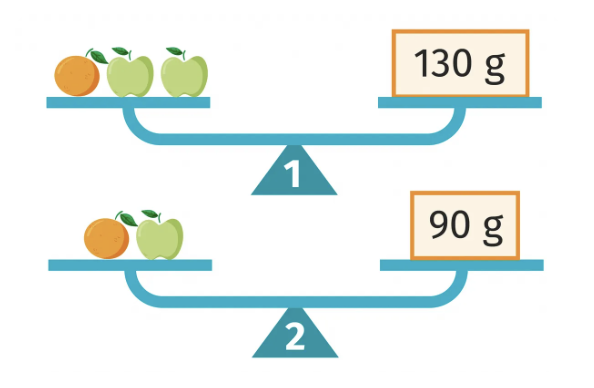
\includegraphics[width=4.5cm]{IMG/balance1}
\end{center}


\end{minipage}


\textbf{Résolution :} On considère la balance n°2 et on ajoute une pomme de chaque côté pour conserver l'équilibre \textcolor{Couleur10}{\textbf{(a)}} Puis, grâce à l'information de la balance n°1, on peut remplacer les fruits du plateau de gauche par une masse de 130 g \textcolor{Couleur10}{\textbf{(b)}} Et enfin, on retire de chaque côté de la balance 90 g. Les plateaux sont toujours équilibrés donc une pomme pèse 40 g \textcolor{Couleur10}{\textbf{(c)}}.




% Les trois étapes de résolution
\begin{center}


\includegraphics[width=13cm]{IMG/balance2}
\end{center}
\vspace{-0.1cm}

\ligne

\end{Exemple}

\subsection*{III. Motifs évolutifs}
\addcontentsline{toc}{subsection}{III. Motifs évolutifs}

Certains motifs admettent une structure qui se répète. On peut alors prévoir la forme d'un motif au bout de plusieurs répétitions.
\vspace{0.2cm}
\begin{Exemple}
\vspace{-1cm}
\begin{minipage}[c]{0.45\textwidth}
On considère le motif ci-contre.

On souhaite connaître le nombre d'allumettes nécessaires à l'étape 32.

\end{minipage} \hfill \begin{minipage}[c]{0.55\textwidth}



% Figure avec les trois étapes
\begin{center}
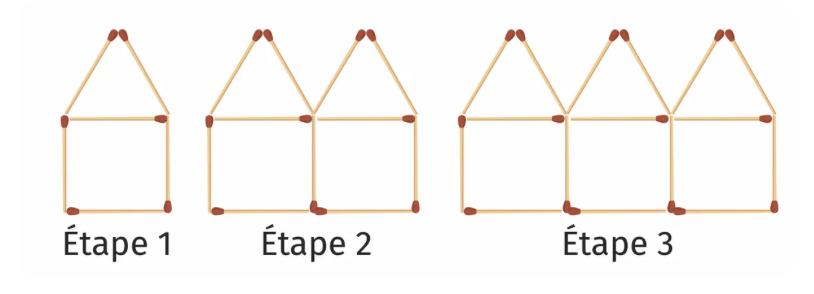
\includegraphics[width=9cm]{IMG/alumette1}
\end{center}
\end{minipage}

\begin{minipage}[c]{0.8\textwidth}
\textbf{Méthode :} Dans ce genre de problème, il ne faut surtout pas écrire toutes les étapes une par une pour répondre à la question, mais repérer la structure qui se répète dans le motif.

Dans cet exemple, on remarque que pour passer de l'étape 1 à l'étape 2, on ajoute cinq allumettes qui correspondent à la structure ci-contre. \end{minipage} \hfill \begin{minipage}[c]{0.2\textwidth}




% Figure avec la structure répétitive
\begin{center}
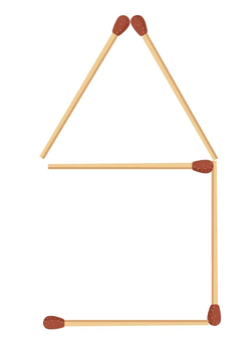
\includegraphics[width=2cm]{IMG/alumette2}
\end{center}
\end{minipage}

\vspace{0.2cm}

\begin{minipage}[c]{0.5\textwidth}
\vspace{0.2cm}

\ligne

\ligne

\ligne

\ligne

\ligne

\ligne

\ligne

\ligne

\ligne

\end{minipage} \hfill \begin{minipage}[c]{0.5\textwidth}

% Tableau avec les étapes et calculs
\setlength{\arrayrulewidth}{1pt} % ou 1.5pt, 3pt selon votre préférence
\arrayrulecolor{Couleur10}
\begin{center}
\renewcommand{\arraystretch}{1.2}
\begin{tabular}{|>{\centering\arraybackslash}p{1.4cm}|>{\centering\arraybackslash}p{4.5cm}|}
\hline
\cellcolor{Couleur10!20} \textbf{Étape} &\cellcolor{Couleur10!20}  \textbf{Nombre d'allumettes} \\
\hline
\textcolor{Couleur10}{\textbf{1}} &  \\
\hline
\textcolor{Couleur10}{\textbf{2}} &  \\
\hline
\textcolor{Couleur10}{\textbf{3}} &  \\
\hline
\textcolor{Couleur10}{\textbf{4}} & \phantom{$6 + 5 + 5 + 5 = 6 + \textcolor{Couleur10}{\textbf{3}} \times 5$} \\
\hline
\textbf{...} & \\
\hline
\textcolor{Couleur10}{\textbf{32}} &  \\
\hline
\end{tabular}
\end{center}
\end{minipage}

\end{Exemple}

\end{document}